% Principle of X-ray photoelectron spectroscopy (XPS)
% Author: Mathias Laurin
\documentclass{article}
\usepackage{tikz}
\usetikzlibrary{decorations.pathmorphing}


\begin{document}
    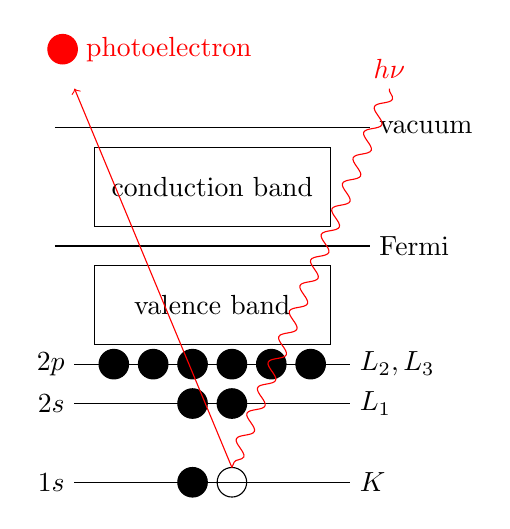
\begin{tikzpicture}[scale=0.25]
    \begin{scope} % Energy levels
        \draw (1,0) node[left] {$1s$} -- 
            ++(14,0) node[right] {$K$};
        \draw (1,4) node[left] {$2s$} -- 
            ++(14,0) node[right] {$L_1$};
        \draw (1,6) node[left] {$2p$} -- 
            ++(14,0) node[right] {$L_2,L_3$};
        \draw (0,12) -- 
            ++(16,0) node[right] {Fermi};
        \draw (0,18) -- 
            ++(16,0) node[right] {vacuum};
    \end{scope}
    \begin{scope} % Valence and conduction bands
        \draw (2,7) rectangle node {valence band} 
            ++(12,4);
        \draw (2,13) rectangle node {conduction band} 
            ++(12,4);
    \end{scope}
    \begin{scope} % Electrons
        \foreach \x in {3,5,...,13}
            \filldraw (\x, 6) circle (.75);
        \foreach \x in {7, 9}
            \filldraw (\x, 4) circle (.75);
        \filldraw (7,0) circle (.75);
        
        %\filldraw(9, 0) circle (.75);
        
        \draw (9, 0) circle (.75);
    \end{scope} 
    \begin{scope}[color=red] % X-rays in, electron out
        \draw[decorate, decoration=snake] (17,20) 
            node[above] {$h\nu$}
            -- (9,0.75);
        \draw[->] (9,0.75) -- (1,20);
        \filldraw (0.4,22) circle (0.75) node[right=5] {photoelectron};
    \end{scope}
        
    \end{tikzpicture}
\end{document}